% \section*{Reproducibility Statement}
% We ensure reproducibility of our work as follows. The prompts used in all experiments are provided in Appendix~\ref{sec:implement_details}, and a complete list of hyperparameters is included in Appendix~\ref{sec:hyperparameters}. All datasets and models employed in our experiments are publicly available. In addition, detailed descriptions of dataset modifications and query constructions are documented in Appendix~\ref{sec:implement_details}.


% \section*{The Use of Large Language Models}
% This manuscript was refined with the assistance of LLMs, which were used to improve clarity, grammar, and overall readability. The use of these models was restricted to language editing and did not influence the scientific content.
\section{Complexity Analysis of the Subgraph Retriever}\label{sec:complexity}
\subsection{Subgraph Selection}
Computing the $k$-hop neighborhood for a single seed $e_i$ can be implemented via a truncated BFS on the undirected projection of the knowledge graph, which takes 
$O(|\mathcal V^k(e_i)| + |\mathcal T^k(e_i)|)$ time.
Aggregating over all $m$ seed entities, the total time complexity of subgraph selection is
\[
O\!\left(\sum_{i=1}^{m} \big(|\mathcal V^k(e_i)| + |\mathcal T^k(e_i)|\big)\right).
\]
Maintaining the union of nodes and edges using hash-based data structures incurs only linear overhead in the size of the resulting candidate graph and does not change the asymptotic complexity.

\subsection{Multi-step Graph Pruning}
Computing $\deg(v)$ for all $v\in\mathcal V'$ can be done by a single pass over edges in $\mathcal T'$, which takes $O(|\mathcal T'|)$ time.

\paragraph{Stage 1: Local Pruning.}
Thresholding nodes by $\rho$ requires scanning all nodes once, i.e., $O(|\mathcal V'|)$.
Removing incident edges can be implemented by filtering $\mathcal T'$ in one pass (keeping only edges whose endpoints survive), which costs $O(|\mathcal T'|)$.
Finally, discarding isolated nodes can be done by recomputing degrees on the remaining edge set, adding another $O(|\mathcal T'|)$ (or $O(|\mathcal V'|+|\mathcal T'|)$ with an adjacency list).
Overall, the time complexity of Stage~1 is
\[
O(|\mathcal V'| + |\mathcal T'|).
\]

Note that $\rho$ only affects the size of the retained node/edge sets after pruning; the worst-case running time remains linear in $|\mathcal V'|+|\mathcal T'|$.

\paragraph{Stage 2: Connectivity Guarantee.}
Assume each pruned neighborhood is stored as a hash set.
Then computing one intersection $\mathcal I_{ij}$ takes
$O(\min\{|\mathcal V^k_\rho(e_i)|, |\mathcal V^k_\rho(e_j)|\})$ time by iterating over the smaller set and checking membership in the larger set.
Thus, computing all pairwise intersections costs
\[
O\!\left(\sum_{1\le i<j\le m}\min\Big\{|\mathcal V^k_\rho(e_i)|, |\mathcal V^k_\rho(e_j)|\Big\}\right).
\]
% Let $N_k(\rho)=\max_i |\mathcal V^k_\rho(e_i)|$. 
In the worst case, this is upper bounded by
$
O(m^2\,\max_i |\mathcal V^k_\rho(e_i)|).
$
Building $\mathcal H_\rho$ while checking whether $\mathcal I_{ij}$ is empty is included in the above cost, and checking connectivity of $\mathcal H_\rho$ via BFS/DFS takes
$O(m+|\mathcal T_\rho|)\le O(m^2)$,
where $T_\rho$ is the edges of $\mathcal H_\rho$.
Let
$
N_k(\rho)=\max_i |\mathcal V^k_\rho(e_i)|
$. Hence, the overall per-round time complexity of Stage~2 is dominated by
\[
O(m^2 N_k(\rho)).
\]

Let $R(\rho)$ be the number of relaxation rounds until $\mathcal H_\rho$ becomes connected.
Since each round reruns Stages~1--2, the total time spent on Stage~2 across all rounds is
\[
O\!\left(\sum_{t=1}^{R(\rho)} m^2\,N_k(\rho_t)\right)
\quad\le\quad
O\!\left(m^2 R(\rho)  N_k(\rho^\star))\right),
\]
where $\rho^\star$ denotes the final threshold at which connectivity is restored.

\paragraph{Stage 3: Leaf Entity Pruning.}
This process can be implemented using a queue-based peeling procedure.
We first compute the degree of each node in $O(|\mathcal T_\rho|)$ time, enqueue all non-seed nodes with degree one, i.e., with only one neighbor. and then iteratively remove them while updating the degrees of their neighbors.
Each node is enqueued and removed at most once, and each relation in $\mathcal T_\rho$ is deleted at most once.
Therefore, the total time complexity of Stage~3 is
\[
O\!\left(|\mathcal V_\rho| + |\mathcal T_\rho|\right).
\]

\paragraph{Stage 4: Compactness Control.}
Let $\mathcal I^+=\{\mathcal I_{ij}\mid \mathcal I_{ij}\neq\emptyset\}$ denote the collection of non-empty intersections obtained in Stage~2,
where $\mathcal I_{ij}=\mathcal V^k_\rho(e_i)\cap\mathcal V^k_\rho(e_j)$.
We select a subset $T^c\subseteq \mathcal I^+$ whose index pairs jointly cover all seed entities.
Let $\lambda=|T^c|$ denote the number of selected intersections.

For each $\mathcal I_{ij}\in T^c$, we retain a subset $\hat{\mathcal I}_{ij}\subseteq\mathcal I_{ij}$ of size $s$
corresponding to the entities with the lowest hub penalties.
This operation can be implemented by partial selection (e.g., using a heap of size $s$),
which takes $O(|\mathcal I_{ij}|\log s)$ time. Since 
$
N_k(\rho)=\max_i |\mathcal V^k_\rho(e_i)|$
and $|\mathcal I_{ij}|\le N_k(\rho)$, the total cost of this step is
\[
O\!\left(\sum_{\mathcal I_{ij}\in T^c} |\mathcal I_{ij}|\log s\right)
\le O\big(\lambda\,N_k(\rho)\log s\big).
\]

Next, for each retained set $\hat{\mathcal I}_{ij}$, we perform a truncated $k$-hop expansion restricted to the corresponding
pruned neighborhoods $\mathcal V^k_\rho(e_i)\cup\mathcal V^k_\rho(e_j)$.
This expansion can be implemented as a multi-source BFS and visits each node and relation at most once within the restricted region.
Let
$
T(\rho)=\max_i |\mathcal T^k_\rho(e_i)|
$
denote the maximum number of relations in a pruned $k$-hop neighborhood.
The cost of this expansion is $O(N_k(\rho)+T_k(\rho))$ per intersection,
and $O(\lambda(N_k(\rho)+T_k(\rho)))$ in total.

For each $T^c$, the induced subgraph over the expanded node set is constructed and further simplified using Stage~3.
Both operations are linear in the size of the resulting subgraph and thus do not affect the asymptotic complexity.

Putting everything together, the overall time complexity of Stage~4 is
\[
O\big(\lambda\,N_k(\rho)\log s + \lambda(N_k(\rho)+T_k(\rho))\big).
\]


\paragraph{Stage 5: Iterative Reduction.}
Let $R (s)$ denote the number of reduction rounds, i.e., the number of times Stage~4 is reapplied with decreasing values of $s$.
Since each round invokes Stage~4 once, the total cost of Stage~5 is the sum of the costs across all rounds.
Using the complexity of Stage~4, the overall time complexity of Stage~5 is
\[
O\!\left(
\sum_{t=1}^{R (s)}
\big(
\lambda\,N_k(\rho)\log s_t
+
\lambda(N_k(\rho)+T_k(\rho))
\big)
\right),
\]
where $s_t$ denotes the value of $s$ at the $t$-th reduction round.

In practice, $s$ is initialized to a small constant and monotonically decreased, and $R (s)$ is typically very small.
Therefore, the complexity of Stage~5 is dominated by a constant number of invocations of Stage~4 and remains
\[
O\big(\lambda(N_k(\rho)+T_k(\rho))\big)
\]
up to a small multiplicative factor.


\subsection{Overall Complexity}

We summarize the time complexity of the entire subgraph retrieval and pruning pipeline.
Recall that $m=|\mathcal E_q|$ denotes the number of seed entities.
We denote by
$
N_k(\rho)=\max_i |\mathcal V^k_\rho(e_i)|, \qquad
T_k(\rho)=\max_i |\mathcal T^k_\rho(e_i)|
$
the maximum numbers of nodes and relations in a pruned $k$-hop neighborhood under threshold $\rho$.
Here, $R(\rho)$ denotes the number of threshold relaxation rounds in Stage~2,
$\lambda=|T^c|$ the number of selected intersections in Stage~4,
and $R(s)$ the number of reduction rounds in Stage~5.

Aggregating the costs of all stages, the total time complexity is
\[
T_{\text{total}}
=
O\!\left(
\sum_{i=1}^{m}\big(|\mathcal V^k(e_i)|+|\mathcal T^k(e_i)|\big)
+
m^2\,R(\rho)\,N_k(\rho^*)
+
R(s)\big(\lambda\,N_k(\rho^*)\log s + \lambda(N_k(\rho^*)+T_k(\rho^*))\big)
+
|\mathcal V'_{\rho^*}|+|\mathcal T'_{\rho^*}|
\right),
\]
where $\rho^*$ denotes the final threshold at which connectivity is restored.

We simplify this expression by identifying dominated terms.
First, since $\mathcal V'_{\rho^*}\subseteq \bigcup_{i=1}^m \mathcal V^k_{\rho^*}(e_i)$ and
$\mathcal T'_{\rho^*}\subseteq \bigcup_{i=1}^m \mathcal T^k_{\rho^*}(e_i)$, we have the crude upper bounds
\[
|\mathcal V'_{\rho^*}| \le \sum_{i=1}^m |\mathcal V^k_{\rho^*}(e_i)| \le m\,N_k(\rho^*),
\qquad
|\mathcal T'_{\rho^*}| \le \sum_{i=1}^m |\mathcal T^k_{\rho^*}(e_i)| \le m\,T_k(\rho^*).
\]
Hence the linear pruning terms satisfy
\[
|\mathcal V'_{\rho^*}|+|\mathcal T'_{\rho^*}| = O\big(m\,(N_k(\rho^*)+T_k(\rho^*))\big).
\]
Similarly, the subgraph selection cost can be upper bounded by
\[
\sum_{i=1}^{m}\big(|\mathcal V^k(e_i)|+|\mathcal T^k(e_i)|\big)
= O\big(m\,(N_k(\rho^*)+T_k(\rho^*))\big),
\]
up to a change from $\rho$-pruned neighborhoods to an upper bound.

Second, the term $\lambda\,N_k(\rho^*)\log s$ arises from partial selection within intersections.
In practice $s$ is a small constant, so $\log s = O(1)$ and
\[
\lambda\,N_k(\rho^*)\log s = O(\lambda\,N_k(\rho^*)).
\]

Third, Stage~5 repeats Stage~4 for $R(s)$ rounds with decreasing $s$.
In practice $R(s)$ is typically very small (often a constant), so Stage~5 introduces only a small multiplicative factor.

Combining these observations, and dropping lower-order linear terms that are dominated by the costs in Stage~2 and Stages~4--5,
the overall complexity is dominated by
\[
T_{\text{total}}
=
O\!\left(
m^2\, R(\rho)\,N_k(\rho^*)
+
R(s)\,\lambda\,(N_k(\rho^*)+T_k(\rho^*))
\right).
\]

\subsection{Discussion}
A natural formulation for connecting multiple seed entities is Steiner tree problem.
While Steiner-tree approaches are theoretically appealing, their computational characteristics
and operational assumptions differ substantially from the requirements of query-driven reasoning on large knowledge graphs.
Below we discuss key considerations motivating our design.

\paragraph{Computational complexity.}
Exact Steiner tree computation on general graphs is NP-hard and exhibits exponential dependence on the number of terminals $m$.
Typical exact algorithms, such as dynamic programming over subsets of terminals, have worst-case running time
\[
O\!\left(3^{m}\,|\mathcal V| + 2^{m}\,|\mathcal V|\log|\mathcal V|\right),
\]
which is up to polylogarithmic factors and quickly becomes prohibitive even for moderately sized multi-entity queries.

Approximate or heuristic Steiner methods avoid the exponential dependence on $m$,
but their complexity is typically dominated by repeated shortest-path computations among terminals.
For example, constructing a metric closure by running single-source shortest-path algorithms from each terminal
followed by a minimum spanning tree incurs
\[
O\!\left(m\,(|\mathcal T| + |\mathcal V|\log|\mathcal V|) + m^2\log m\right),
\]
 where the dominant term arises from $m$ shortest-path searches on the (sub)graph.

In contrast, our approach avoids exponential dependence on $m$.
As shown in our analysis, the dominant cost scales as
\[
O\!\left(
R(\rho)\,m^2\,N_k(\rho^*)
+
R(s)\,\lambda\,(N_k(\rho^*)+T_k(\rho^*))
\right),
\]
which is polynomial in $m$ and bounded by the sizes of pruned $k$-hop neighborhoods.

\textbf{Locality of computation.}
A key distinction lies in the scope of computation.
Steiner-based formulations typically rely on shortest-path searches whose cost is tied to global graph structure.
In contrast, all major operations in our framework: pairwise intersections, connectivity checks,
and compactness control—are confined to pruned local neighborhoods
$\mathcal V^k_{\rho^*}(e_i)$ and their unions.
Consequently, the complexity is governed by $N_k(\rho^*)$ and $T_k(\rho^*)$ rather than global graph statistics.

\textbf{Controlled trade-off between connectivity and compactness.}
Our method exposes explicit parameters $(\rho,k,\lambda,s)$ that directly regulate the trade-off
between connectivity and compactness.
The threshold $\rho$ and the number of relaxation rounds $R(\rho)$ control how aggressively neighborhoods are pruned,
while $\lambda$ and $s$ bound the number and size of retained intersections.
This results in a predictable and tunable computational budget at query time.
By contrast, Steiner-tree formulations do not provide similarly explicit query-level controls over the explored subgraph size.

\textbf{Pairwise interactions versus global optimization.}
Although our approach involves a quadratic dependence on $m$ due to pairwise interactions among seed entities,
these interactions are limited to set intersections and bounded neighborhood expansions.
This is fundamentally different from global optimization objectives in Steiner-tree formulations,
where pairwise relationships are mediated through shortest-path computations over large graphs.
As a result, the quadratic term in our method remains tractable in practice and does not introduce super-polynomial behavior.



\section{Details of Experiments}

\subsection{Hyperparameters}\label{sec:hyperparameters}
Table~\ref{tab:hyperparameters} summarizes the key hyperparameters used in our experiments.

\begin{table}[h]
\centering
\caption{Hyperparameter settings used across all experiments.}
\resizebox{0.5\textwidth}{!}{%
\begin{tabular}{ll}
\toprule
\textbf{Category} & \textbf{Setting} \\
\midrule
\multicolumn{2}{l}{\textbf{Data / Input Configuration}} \\
Max Prompt Length        & 8192 \\
Max Response Length      & 2048 \\
Validation Batch Size    & 1024 \\
Random Seed              & 1 \\
\midrule
\multicolumn{2}{l}{\textbf{Optimization}} \\
Global Batch Size (Actor/Critic) & 64 \\
Learning Rate            & $1 \times 10^{-6}$ \\
Weight Decay             & $1 \times 10^{-2}$ \\
Optimizer                & AdamW (bf16) \\
Max Gradient Norm        & 1.0 \\
\midrule
\multicolumn{2}{l}{\textbf{Rollout Configuration}} \\
Number of Rollouts       & 5 (train), 1 (validation) \\
Rollout Temperature      & 1.0 (train), 0.6 (validation) \\
Rollout Top-$p$          & 1.0 (train), 0.95 (validation) \\
Max Batched Tokens       & 10240 \\
\midrule
\multicolumn{2}{l}{\textbf{KL Control}} \\
KL Coefficient ($\lambda_{KL}$) & $1 \times 10^{-2}$ \\
\midrule
\multicolumn{2}{l}{\textbf{Training Setup}} \\
Total Epochs             & 20 (2-entities), 40 (3-/4-entities) \\
\bottomrule
\end{tabular}
}
\label{tab:hyperparameters}
\end{table}


\subsection{Implementation Details}\label{sec:implement_details}

\paragraph{Datasets} Table~\ref{tab:datasets} summarizes the datasets used in our experiments, including their sources, number of entities, and number of triples. 
For FB15k-237, we replace machine identifiers with their corresponding human-readable entity names. 
To address the issue of long and complex relation names in Freebase, we transform each relation into a simplified alias with the assistance of ChatGPT, followed by manual verification. 
For example, the original relation \texttt{/film/actor/film./film/performance/film} is shortened to \texttt{acted\_in}.


\begin{table*}[ht]
\centering
\caption{Statistics of knowledge graph datasets.}
\resizebox{0.82\textwidth}{!}{%
\begin{tabular}{l l r r r}
\toprule
\textbf{Datasets} & \textbf{Source} & \textbf{\#Entities} & \textbf{\#Relations} & \textbf{\#Triples} \\
\midrule
\textbf{Freebase13}   & Freebase & 75,043  & 13  & 375,514 \\
\textbf{FB15k-237}    & Freebase & 14,265  & 237 & 310,116 \\
\textbf{MetaQA}       & Movie-domain & 40,151 & 9   & 134,741 \\
\textbf{DBpedia50}    & Subset of DBpedia (Wikipedia) & 30,449 & 365 & 43,756 \\
\textbf{DBpedia500}   & Larger subset of DBpedia & 490,598 & 573 & 4,268,614 \\
\textbf{YAGO3-10}     & Subset of YAGO3 (Wikipedia, WordNet, GeoNames) & 123,182 & 37 & 1,089,040 \\
\textbf{UMLS}         & Unified Medical Language System & 135 & 46 & 6,529 \\
\bottomrule
\end{tabular}
}

\label{tab:datasets}
\end{table*}


\paragraph{Query Construction} 
For \textit{two-entity} queries, we sampled pairs of seed entities 
such that the shortest path distance $\mathrm{dist}(e_i, e_j) \leq 4$ in knowledge graph. 
The sampling procedure (Algorithm~\ref{alg:sample_pair}) performs repeated random selection of a source entity 
and then selects a target entity reachable within $k$ hops. 
This ensures that queries follow the graph’s local connectivity.

\begin{algorithm}[ht]
\caption{Entity Pair Sampling}
\label{alg:sample_pair}
\begin{algorithmic}[1]
\STATE Randomly sample an entity $u$ from the graph.
\STATE Run BFS up to $k$ hops to obtain reachable set $\mathcal{N}(u,k)$.
\STATE Randomly sample $v \in \mathcal{N}(u,k)$ with $d(u,v)\leq k$.
\STATE Return $(u,v)$ as the entity pair.
\end{algorithmic}
\end{algorithm}


To evaluate scalability, we further constructed queries involving \textit{three} and \textit{four} entities 
on the DBpedia50 dataset. 
For triplets $(u,v,w)$, we required that the third entity $w$ 
is within $k$ hops of at least one of the first two entities ($u$ \textit{or} $v$). 
For quadruplets $(u,v,w,z)$, we extended this requirement so that 
the fourth entity $z$ is within $k$ hops of at least one of $\{u,v,w\}$. 
This OR-connectivity guarantees that multi-entity queries yield semantically well-connected subgraphs.

After sampling seed entities, we converted them into natural language questions 
using a set of manually designed templates. 
For example, given the pair (\textit{Meghan Markle}, \textit{Queen Elizabeth II}), 
we generate the query: 
\textit{``How are Meghan Markle and Queen Elizabeth II associated?''} 
We also used alternative phrasings such as 
\textit{``For what reason are [entity1] and [entity2] related?''} 
to improve linguistic diversity. 

\paragraph{Prompts} For each experiment, we constructed prompts that contextualize the knowledge graph and the query into a unified text input.  
Specifically, the graph is represented as \textbf{node and edge tables}, followed by the natural language query, together with task-specific instructions.  
This design ensures that the model has access to both structural and semantic information.  

An example prompt is shown below.
{\small
\begin{verbatim}
You are given a directed graph as two CSV-like sections in this order:

1) Node table (header included):
node_id, node_attr

2) Edge table (header included):
src, edge_attr, dst

Task
- Use ONLY edges from the Edge table to answer the question by outputting 
  a path.
- When printing each edge, replace IDs with the exact node_attr from the 
  Node table.
- Output MUST be text triples, not numeric IDs.

Output format (STRICT — no extra text):
GRAPH:
("subject"|predicate|"object")
...
END

Rules
- Use only listed edges; do NOT invent edges.
- Map IDs → node_attr; preserve node_attr exactly.
- Output NOTHING outside the SUBGRAPH block.
- If no subgraph exists, output exactly:
GRAPH:
END

Graph:
node_id, node_attr
1, Meghan Markle
2, Prince Harry
3, Prince William
4, Queen Elizabeth II

src, edge_attr, dst
1, spouse, 2
4, grandmother, 2
4, grandmother, 3
2, brother, 3

Question: How are Meghan Markle and Queen Elizabeth II associated?

Your output must be ONLY the SUBGRAPH block.
\end{verbatim}
}

\paragraph{Additional Evaluation Metrics}
Besides the three primary metrics, Connectivity Ratio, Average Reward, and Subgraph F1, 
we report additional reward components to provide a more fine-grained evaluation of relational answers.

\noindent
\textbf{Subgraph F1.}
Subgraph F1 evaluates the overlap between a predicted relational answer and the ground-truth answer subgraph at the triple level.
We define precision and recall over triples, and compute F1 as their harmonic mean:
\begin{equation}
\label{eq:subgraph_f1}
\mathrm{Precision} = \frac{|T_p \cap T_{gt}|}{|T_p|}, \quad
\mathrm{Recall} = \frac{|T_p \cap T_{gt}|}{|T_{gt}|}, \quad
\mathrm{F1} = \frac{2 \cdot \mathrm{Precision} \cdot \mathrm{Recall}}{\mathrm{Precision} + \mathrm{Recall}},
\end{equation}
where $T_p$ and $T_{gt}$ denote the sets of RDF triples in the predicted and ground-truth subgraphs, respectively.

\noindent
In addition to these primary metrics, we report the following reward components:

\squishlist
  \item \textit{Correct Format Percentage} ($F$): the proportion of generated subgraphs that conform to the required output format.
  \item \textit{Average Entity Informativeness} ($I_E$): the \textit{negative} of the average informativeness score of entities (Equation~\ref{eq:entity_informativenss}); lower values indicate more informative entities.
  \item \textit{Average Relation Informativeness} ($I_R$): the \textit{negative} of the average informativeness score of relations (Equation~\ref{eq:relation_informativenss}); lower values indicate more informative relations.
\squishend

\noindent
Note that \textit{Average Entity Informativeness} and \textit{Average Relation Informativeness} are only available when the format reward equals 1 and the generated subgraph is connected.
Therefore, for two-entity queries, we compute these averages only over the connected answers.





\subsection{Details of Main Results}\label{sec:main_results_details}

\paragraph{Parameter Choice.}

\begin{table}[ht]
\centering
\renewcommand{\arraystretch}{1.2}
\caption{Evaluation results of Qwen-2.5-3B-Instruct model on DBpedia500 under different parameter settings. Only reachable cases are reported for $I_R$ and $I_E$.}
\setlength{\tabcolsep}{8pt}
\resizebox{0.4\textwidth}{!}{%
\begin{tabular}{cc c c c c}
\toprule
\textbf{$x$} & \textbf{$y$} & \textbf{$F$} & \textbf{$C$} & \textbf{$I_R$} & \textbf{$I_E$} \\
\midrule
5 & 4 & 100.0\% & 59.0\% & -5.12 & -5.84 \\
6 & 5 & 100.0\% & 60.6\% & -5.62 & -6.43 \\
7 & 6 & 100.0\% & 64.8\%& -5.83 & -7.24 \\
8 & 7 & 100.0\% & 64.2\% & -6.39 & -7.95 \\
\bottomrule
\end{tabular}
}
\label{tab:dbpedia500_results}
\end{table}

For the normalization terms $y$ and $x$ in Equation~\ref{eq:reward}, 
we calibrated their values using the Qwen-2.5-3B-Instruct model on the largest dataset, DBpedia500. 
Since the shortest distance between entity pairs is bounded by $\mathrm{dist}(e_i,e_j) \leq 4$, 
the optimal case for two-entity queries typically involves about four relations and five entities. 
Accordingly, we initialized the parameter search from $(x,y)=(5,4)$.  

Table~\ref{tab:dbpedia500_results} presents the evaluation across different $(x,y)$ values. 
Transitioning from $(5,4)$ to $(6,5)$ leads to a marginal improvement in Connectivity Ratio of 1.6\%, 
but this gain is offset by a reduction in informativeness, with $I_R$ decreasing by 0.50 and $I_E$ by 0.59, 
resulting in a total loss of 1.09. 
By comparison, $(7,6)$ achieves the highest Connectivity Ratio of 64.8\%, representing a 4.2\% increase over $(6,5)$, 
while the informativeness loss remains essentially identical: $I_R$ decreases by 0.21 and $I_E$ by 0.81, 
again summing to 1.09. 
This outcome highlights that $(7,6)$ delivers a substantially better trade-off, 
offering a larger connectivity gain without incurring additional informativeness penalties. 
When further increasing the parameters to $(8,7)$, the Connectivity Ratio ceases to improve and instead begins to decline.  

Based on these observations, we selected $(y,x)=(7,6)$ as the final configuration. 
These values were fixed and applied uniformly across all datasets and models with two-entity queries 
to ensure consistency and comparability.




\paragraph{Performance Comparison across Models and Datasets.}
Table~\ref{tab:main_additional_results} reports the average relation and entity informativeness of Prompting and UniRel across datasets, where lower values indicate more informative relations or entities.

\begin{table*}[ht]
\centering
\caption{Average relation and entity informativeness of Prompting and UniRel where each tuple represents ($I_R$, $I_E$).} 
\resizebox{0.8\textwidth}{!}{%
\begin{tabular}{llccccccc}
\toprule
\multicolumn{2}{c}{\diagbox{\textbf{Models}}{\textbf{Datasets}}} & \textbf{Freebase13} & \textbf{FB15k-237} & \textbf{MetaQA} & \textbf{DBpedia50} & \textbf{DBpedia500} & \textbf{YAGO3-10} & \textbf{UMLS} \\
\midrule
\multirow{2}{*}{\textbf{Qwen3B}}          
& Prompting    & (0.59, 0.67) & (1.93, 1.93) & (1.19, 1.12) & (0.91, 0.53) & (1.31, 1.225) & (0.60, 0.26) & (1.08, 1.61) \\
& UniRel  & (0.34, 0.94) & (2.97, 2.28) & (2.90, 2.45) & (2.01, 1.78) & (3.109, 4.04) & (2.78, 4.69) & (1.25, 4.78) \\ 
\multirow{2}{*}{\textbf{Qwen7B}}          
& Prompting    & (0.32, 0.75) & (1.63, 1.79) & (2.52, 1.63) & (1.07, 0.71) & (2.14, 1.519) & (1.88, 1.43) & (1.10, 2.06) \\
& UniRel  & (0.36, 1.19) & (2.01, 2.84) & (2.90, 2.71) & (2.02, 1.79) & (3.12, 4.20) & (2.81, 4.81) & (1.34, 6.26) \\ 
\multirow{2}{*}{\textbf{Qwen14B}}        
& Prompting    & (0.33, 0.87) & (2.06, 2.52) & (1.93, 0.50) & (1.46, 1.05) & (3.00, 3.00) & (1.82, 1.84) & (1.38, 2.58) \\
& UniRel  & (0.35, 1.20) & (1.69, 4.18) & (2.78, 3.81) & (1.99, 1.98) & (2.99, 5.19) & (2.46, 5.68) & (1.42, 6.71) \\ 
\midrule
\multirow{2}{*}{\textbf{Llama3B}}         
& Prompting    & (-, -) & (-, -) & (-, -) & (-, -) & (-, -) & (-, -) & (-, -) \\
& UniRel  & (0.35, 1.23) & (2.14, 2.87) & (2.14, 2.87) & (1.89, 1.69) & (3.05, 4.22) & (2.89, 4.57) & (0.62, 1.58) \\ 
\multirow{2}{*}{\textbf{Llama8B}}         
& Prompting    & (0.07, 3.07) & (3.87, 6.82) & (-, -) & (-, -) & (-, -) & (4.17, 11.62) & (-, -) \\
& UniRel  & (0.36, 1.29) & (1.97, 4.23) & (1.97, 4.23) & (2.02, 1.96) & (3.03, 5.78) & (2.78, 6.08) & (1.43, 6.83) \\ 
\midrule
\rowcolor{blue!10}
\multicolumn{2}{l}{\textbf{Optimal Search}} 
& (0.29, 0.77) & (1.12, 1.86) & (2.66, 1.78) & (2.08, 1.45) & (2.58, 1.92) & (2.526, 1.67) & (0.91, 1.93) \\
\bottomrule
\end{tabular}
}
\label{tab:main_additional_results}
\end{table*}

For Prompting, the connected answers are typically simple subgraphs with shorter lengths, which explains the relatively low initial scores. After applying UniRel, additional relations and entities may be introduced to ensure connectivity, which can increase the informativeness scores compared to the optimal baseline.

Compared with the optimal search, certain datasets (e.g., Llama-8B on DBpedia50) exhibit lower $I_R$ but higher $I_E$, revealing a gap between relation- and entity-level informativeness. By contrast, datasets with larger reward gaps from the optimal (e.g., FB15k-237) often show a small difference in $I_R$ but a large difference in $I_E$, suggesting that extra high-degree or hub-penalty entities were included to achieve connectivity.

\begin{table*}[ht]
\centering
\caption{Correct format percentage of Prompting and UniRel.} 
\resizebox{0.8\textwidth}{!}{%
\begin{tabular}{llccccccc}
\toprule
\multicolumn{2}{c}{\diagbox{\textbf{Models}}{\textbf{Datasets}}} & \textbf{Freebase13} & \textbf{FB15k-237} & \textbf{MetaQA} & \textbf{DBpedia50} & \textbf{DBpedia500} & \textbf{YAGO3-10} & \textbf{UMLS} \\
\midrule
\multirow{2}{*}{\textbf{Qwen3B}}          
& Prompting   & 83.6\% & 78.8\% & 84.6\% & 84.6\% & 78.2\% & 78.0\% & 93.0\% \\
& UniRel & 100.0\% & 99.8\% & 95.4\% & 100.0\% & 99.8\% & 100.0\% & 100.0\% \\ 
\multirow{2}{*}{\textbf{Qwen7B}}          
& Prompting   & 96.6\% & 93.8\% & 89.4\% & 95.0\% & 90.0\% & 86.8\% & 88.8\% \\
& UniRel & 100.0\% & 100.0\% & 95.8\% & 100.0\% & 100.0\% & 100.0\% & 100.0\% \\ 
\multirow{2}{*}{\textbf{Qwen14B}}        
& Prompting   & 93.4\% & 91.2\% & 94.0\% & 88.2\% & 85.4\% & 94.2\% & 93.8\% \\
& UniRel & 100.0\% & 100.0\% & 95.6\% & 100.0\% & 100.0\% & 100.0\% & 100.0\% \\ 
\midrule
\multirow{2}{*}{\textbf{Llama3B}}         
& Prompting   & 1.6\% & 1.6\% & 4.2\% & 0.4\% & 3.8\% & 3.4\% & 3.8\% \\
& UniRel & 100.0\% & 99.8\% & 99.8\% & 100.0\% & 100.0\% & 100.0\% & 100.0\% \\ 
\multirow{2}{*}{\textbf{Llama8B}}         
& Prompting   & 4.4\% & 12.6\% & 10.2\% & 2.0\% & 16.6\% & 24.6\% & 4.6\% \\
& UniRel & 100.0\% & 100.0\% & 100.0\% & 100.0\% & 100.0\% & 100.0\% & 100.0\% \\ 
\bottomrule
\end{tabular}
}
\label{tab:format_results}
\end{table*}

Table~\ref{tab:format_results} further reveals that Qwen models exhibit a stronger ability to follow prompt instructions under Prompting, maintaining relatively high correct format percentages (often above 80\%).
In contrast, Llama models struggle to produce valid outputs in the absence of structural guidance, with correct format rates frequently below 5\%.
With UniRel, however, both families achieve nearly perfect compliance across all datasets, indicating that reinforcement-guided adaptation is highly effective in enforcing structural answers.

\begin{table*}[ht]
\centering
\caption{Recall and Precision of Prompting and UniRel where each tuple represents (recall, precision).} 
\resizebox{0.8\textwidth}{!}{%
\begin{tabular}{llccccccc}
\toprule
\multicolumn{2}{c}{\diagbox{\textbf{Models}}{\textbf{Datasets}}} & \textbf{Freebase13} & \textbf{FB15k-237} & \textbf{MetaQA} & \textbf{DBpedia50} & \textbf{DBpedia500} & \textbf{YAGO3-10} & \textbf{UMLS} \\
\midrule
\multirow{2}{*}{\textbf{Qwen-3B}}
& Prompting
& (29.9, 29.1) & (0.5, 0.5) & (5.0, 5.0) & (14.9, 17.6)
& (2.9, 4.9) & (3.9, 4.4) & (13.9, 10.8) \\
& UniRel
& (59.3, 58.2) & (3.6, 2.2) & (25.8, 24.4) & (39.7, 38.8)
& (15.4, 13.7) & (16.6, 15.2) & (17.3, 17.0) \\

\multirow{2}{*}{\textbf{Qwen-7B}}
& Prompting
& (47.6, 40.1) & (0.9, 1.0) & (8.6, 13.4) & (24.0, 29.0)
& (6.5, 10.7) & (8.0, 10.4) & (15.7, 12.1) \\
& UniRel
& (60.8, 59.8) & (3.7, 3.2) & (27.0, 26.4) & (41.0, 40.0)
& (17.1, 15.3) & (18.5, 17.3) & (17.7, 17.6) \\

\multirow{2}{*}{\textbf{Qwen-14B}}
& Prompting
& (54.3, 43.6) & (2.0, 1.9) & (14.1, 20.4) & (30.4, 36.8)
& (9.3, 13.0) & (11.3, 12.7) & (15.7, 12.1) \\
& UniRel
& (63.7, 61.1) & (4.1, 3.5) & (28.4, 27.9) & (44.2, 43.5)
& (17.2, 16.7) & (18.3, 17.7) & (16.7, 16.7) \\

\midrule
\multirow{2}{*}{\textbf{Llama-3B}}
& Prompting
& (0.0, 0.0) & (0.0, 0.0) & (0.0, 0.0) & (0.0, 0.0)
& (0.0, 0.0) & (0.0, 0.0) & (0.0, 0.0) \\
& UniRel
& (62.6, 59.8) & (3.4, 2.6) & (28.0, 26.1) & (27.1, 26.5)
& (13.4, 12.5) & (14.3, 14.3) & (15.4, 15.6) \\

\multirow{2}{*}{\textbf{Llama-8B}}
& Prompting
& (0.0, 0.0) & (0.0, 0.0) & (0.0, 0.0) & (0.0, 0.0)
& (0.0, 0.0) & (0.0, 0.0) & (0.0, 0.0) \\
& UniRel
& (65.7, 64.9) & (4.6, 3.8) & (27.5, 26.8) & (43.2, 42.2)
& (18.6, 17.6) & (19.2, 18.5) & (17.9, 17.8) \\

\bottomrule
\end{tabular}
}
\label{tab:main_additional_results_recall}
\end{table*}



Table~\ref{tab:main_additional_results_recall} reports the triple-level recall and precision of Prompting and UniRel across multiple knowledge graph benchmarks.
Across the evaluated benchmarks, UniRel generally achieves higher recall and precision than Prompting.
Notably, the gains are not limited to recall alone. UniRel also achieves higher precision, suggesting that the recovered triples are not only more complete but also more accurate, rather than being obtained through indiscriminate expansion.
Furthermore, the improvements persist as model size increases, indicating that UniRel complements model scaling by providing better structural guidance instead of relying solely on increased model capacity.





\paragraph{Case Study.}  
We present three additional case studies to further illustrate the differences between the smallest subgraph and the UniRel.  

\begin{figure*}[ht]
    \centering
    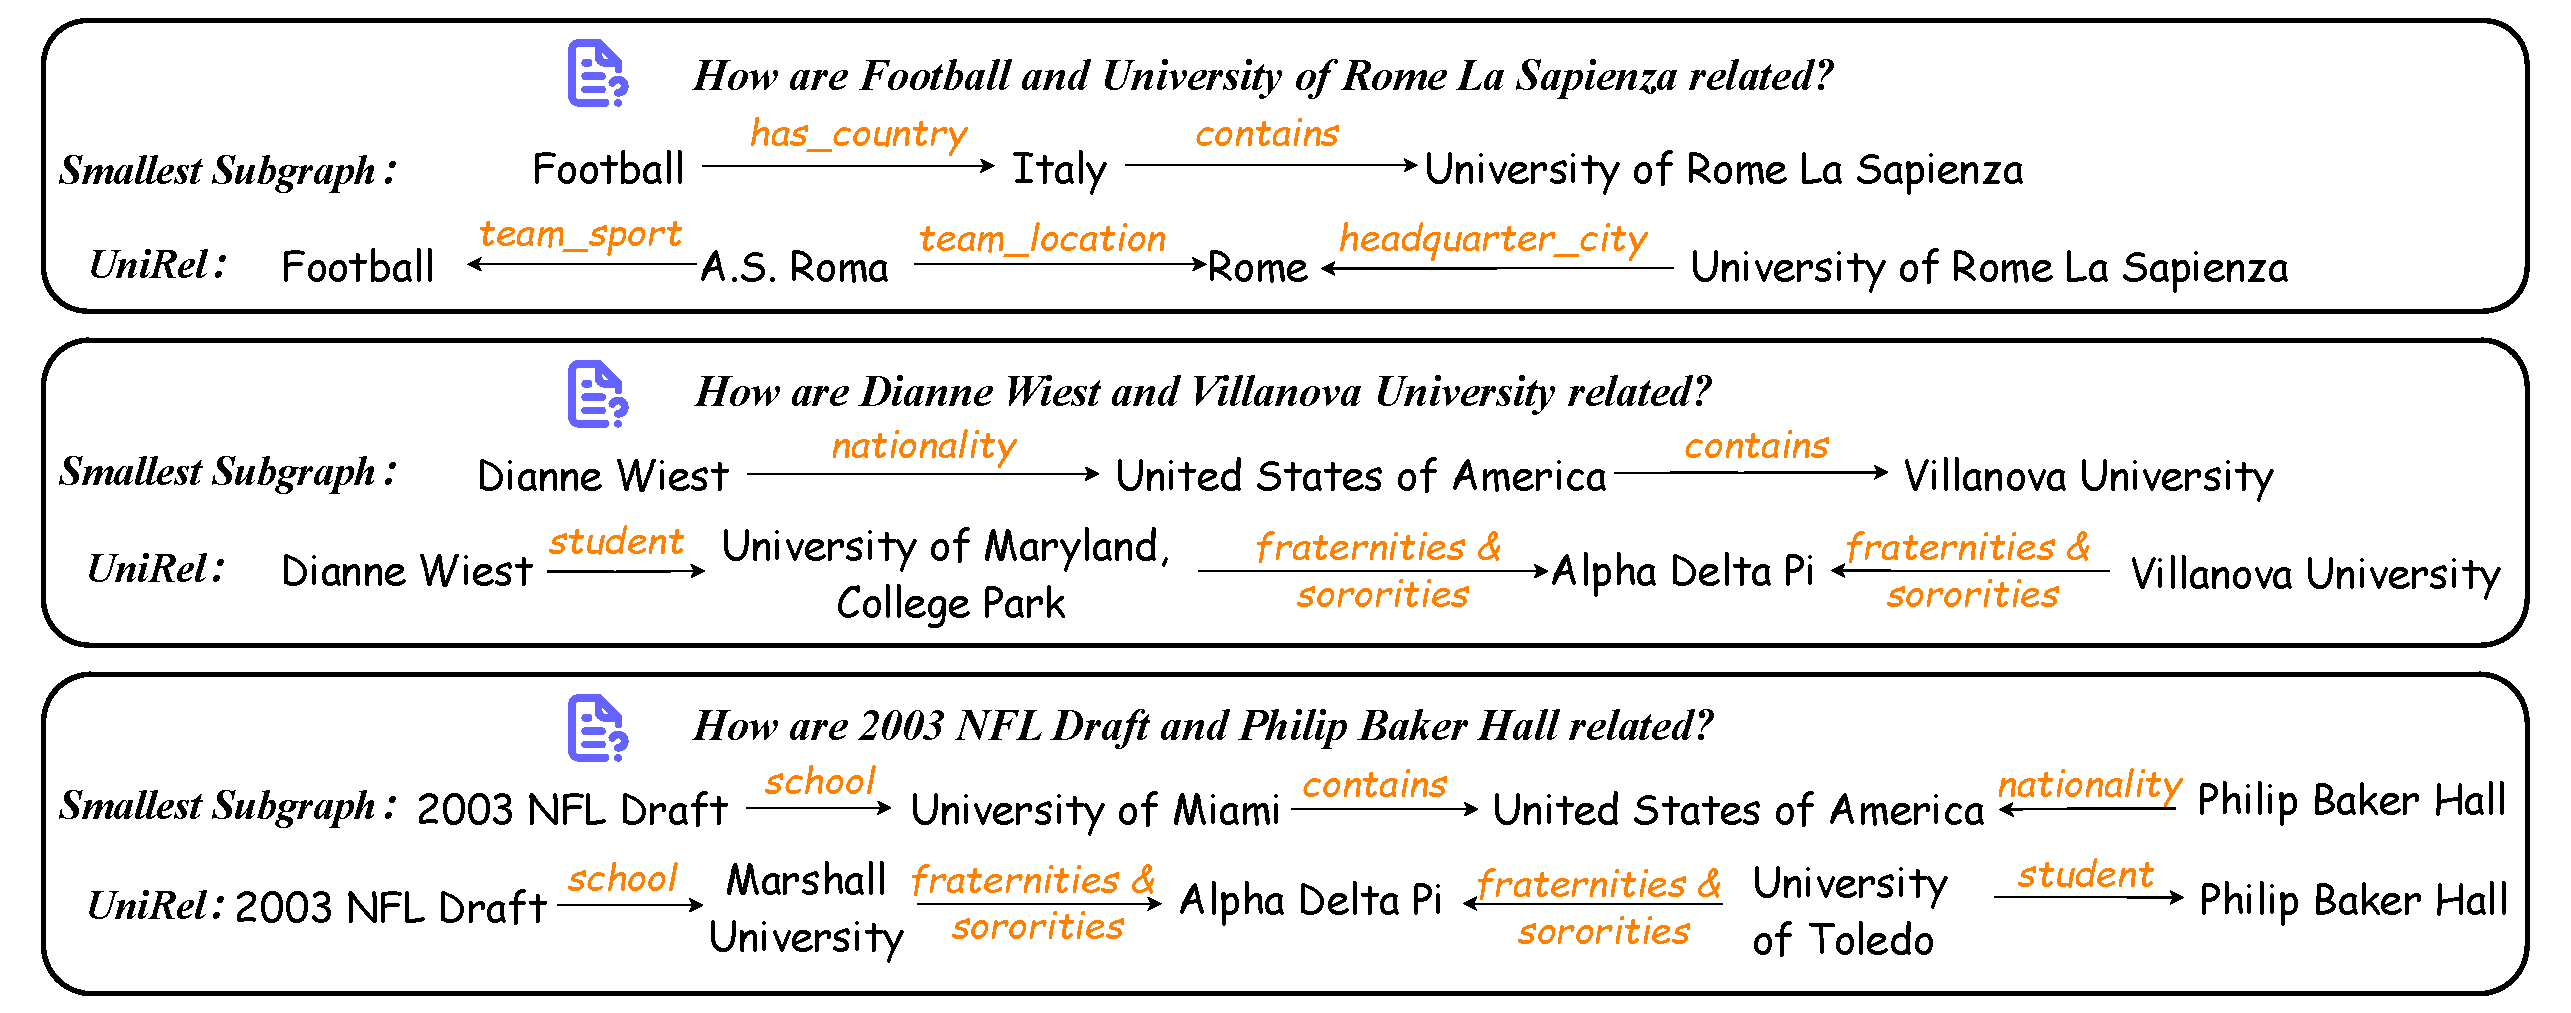
\includegraphics[width=0.95\textwidth]{figures/case_study_2.pdf} 
    \label{fig:case_studies_2}
\vspace{-1em}
\end{figure*}


\subsection{Details of Generalization Results}\label{sec:generalization_results_details}

Table~\ref{tab:generalization_results_complete} reports the complete cross-dataset generalization results of UniRel trained on DBpedia500 and evaluated on all benchmarks.
Beyond the partial results discussed in the main paper, we provide additional analysis to better understand the observed performance variations across datasets.

We observe that generalization performance is relatively strong on DBpedia50, which may be attributed to its high similarity to the training dataset, DBpedia500, in terms of data source, schema, and graph structure.
Both datasets are derived from DBpedia and share similar entity types, relation distributions, and structural patterns, which likely facilitates knowledge transfer under the UniRel framework.

In contrast, generalization performance on UMLS is comparatively weaker.
A possible explanation is the substantial semantic gap between UMLS and DBpedia-based datasets.
UMLS focuses on biomedical concepts and relations that differ significantly from the general-domain entities and relations seen during training.
As a result, semantic similarity learned during pretraining and fine-tuning may be less effective in supporting cross-dataset transfer, limiting the benefits of semantic generalization.

Taken together, these observations suggest that cross-dataset generalization under UniRel is influenced by both semantic similarity and structural compatibility between the training and target knowledge graphs.
Datasets that are closer to the training domain in terms of semantics and structure tend to exhibit stronger transfer performance, while datasets with larger semantic shifts pose greater challenges.


\begin{table*}[ht]
\centering
\caption{Cross-dataset generalization of UniRel trained on DBpedia500, reported as (connectivity ratio, average reward, subgraph F1).}
\resizebox{0.9\textwidth}{!}{%
\begin{tabular}{llccccc}
\toprule
\multicolumn{2}{c}{\diagbox{\textbf{Datasets}}{\textbf{Models}}} & \textbf{Qwen3B} & \textbf{Qwen7B} & \textbf{Qwen14B} & \textbf{Llama3B} & \textbf{Llama8B} \\
\midrule
\multirow{2}{*}{\textbf{Freebase13}} 
 & \cellcolor{gray!12}Original & (80.0\%, 0.52, 44.7) & (83.4\%, 0.59, 46.1) & (94.0\%, 0.77, 52.7) & (81.8\%, 0.55, 46.9) & (91.0\%, 0.72, 54.1) \\
 & \cellcolor{yellow!12}Modified & (69.6\%, 0.33, 41.3) & (74.8\%, 0.43, 44.2) & (84.0\%, 0.60, 50.4) & (81.6\%, 0.55, 46.9) & (87.0\%, 0.65, 51.2) \\
\midrule
\multirow{2}{*}{\textbf{FB15k-237}}  
 & \cellcolor{gray!12}Original & (47.0\%, -0.23, 1.8) & (61.6\%, 0.01, 1.7) & (76.6\%, 0.16, 3.1) & (45.6\%, -0.28, 1.6) & (69.8\%, 0.08, 2.8) \\
 & \cellcolor{yellow!12}Modified & (20.8\%, -0.71, 0.4) & (41.4\%, -0.32, 1.2) & (52.4\%, -0.12, 1.8) & (45.8\%, -0.25, 1.7) & (59.4\%, -0.03, 1.9) \\
\midrule
\multirow{2}{*}{\textbf{MetaQA}}     
 & \cellcolor{gray!12}Original & (60.6\%, -0.12, 20.0) & (69.8\%, 0.04, 21.7) & (78.0\%, 0.11, 23.1) & (64.2\%, -0.06, 21.7) & (80.0\%, 0.18, 23.9) \\
 & \cellcolor{yellow!12}Modified & (29.2\%, -0.56, 9.1)  & (49.0\%, -0.21, 16.5)  & (60.8\%, -0.02, 18.4)  & (67.2\%, 0.06, 22.5) & (72.6\%, 0.15, 23.2) \\
\midrule
\multirow{2}{*}{\textbf{DBpedia50}}  
 & \cellcolor{gray!12}Original & (91.4\%, 0.55, 40.1) & (96.6\%, 0.64, 42.1) & (97.6\%, 0.66, 42.3) & (56.8\%, -0.02, 34.8) & (98.2\%, 0.66, 42.5) \\
 & \cellcolor{yellow!12}Modified & (54.6\%, -0.06, 34.0) & (73.0\%, 0.27, 37.9) & (84.0\%, 0.45, 40.7) & (84.6\%, 0.45, 38.8) & (91.8\%, 0.57, 41.7) \\
\midrule
\multirow{2}{*}{\textbf{YAGO3-10}}   
 & \cellcolor{gray!12}Original & (56.6\%, -0.18, 11.5) & (67.4\%, 0.01, 13.2) & (80.6\%, 0.15, 15.0) & (44.8\%, -0.36, 10.1) & (83.0\%, 0.18, 15.8) \\
 & \cellcolor{yellow!12}Modified & (23.6\%, -0.66, 7.23) & (41.4\%, -0.34, 10.0) & (48.2\%, -0.24, 11.4) & (44.6\%, -0.31, 10.5) & (62.2\%, -0.03, 13.8) \\
\midrule
\multirow{2}{*}{\textbf{UMLS}}       
 & \cellcolor{gray!12}  Original & (49.0\%, -0.19, 13.3) & (55.8\%, -0.07, 13.6) & (74.0\%, 0.10, 12.7)          & (56.4\%, -0.12, 13.4) & (66.6\%, 0.05, 13.1) \\
 \multirow{0}{*}{}
 &\cellcolor{yellow!12} Modified & (41.0\%, -0.30, 13.1) & (43.4\%, -0.24, 13.4) & (50.0\%, -0.14, 12.1) & (49.4\%, -0.17, 13.6) & (55.0\%, -0.07, 12.4) \\
\bottomrule
\end{tabular}
}
\label{tab:generalization_results_complete}
\end{table*}

\subsection{Details of UniRel for Entity-Centric KGQA}\label{sec:entity_centric_results_details}

\paragraph{Datasets.}

We evaluate UniRel on two widely used multi-hop KGQA benchmarks, WebQSP and CWQ as shown in Table~\ref{tab:dataset_stats}.
Both datasets are built on Freebase and require reasoning over multiple entities and relations, making them well suited for evaluating relation-centric and subgraph-based reasoning methods.

WebQSP focuses on relatively constrained multi-hop questions, where answers can often be derived from compact subgraphs connecting a small number of entities.
In contrast, CWQ contains more complex questions with longer reasoning chains and more diverse relational structures, posing greater challenges for subgraph extraction and relational reasoning.



\begin{table}[ht]
\centering
\small
\caption{Dataset statistics.}
\begin{tabular}{lccc}
\toprule
\textbf{Dataset} & \textbf{\#Train} & \textbf{\#Test} & \textbf{Max Hop} \\
\midrule
WebQSP & 2{,}826 & 1{,}628 & 2 \\
CWQ    & 27{,}639 & 3{,}531 & 4 \\
\bottomrule
\end{tabular}
\label{tab:dataset_stats}
\end{table}


\paragraph{Metrics.}
\textbf{F1}: measures the overlap between the predicted answer set and the ground-truth answer set by combining precision and recall.
It reflects how well the model balances answer correctness and completeness, and is particularly suitable for questions with multiple correct answers.

\textbf{Hit@1}: measures whether the top-ranked predicted answer exactly matches the ground-truth answer.
It captures the model’s ability to place the correct answer at the highest rank and is commonly used for single-answer or ranking-based evaluation.
